In questo capitolo discuteremo del processo di integrazione, della qualità dei dati contenuti nei dataset utilizzati prima e dopo il processo di integrazione, infine verranno proposte delle analisi descrittive effettuate sui dati integrati. 
\section{Descrizione dei dataset}
Come accennato nella Sezione \ref{sec:design}, i tre dataset utilizzati, presenti nella \href{https://gitlab.com/Daniele-Papetti/kickstarterprediction}{repository online}, sono stati reperiti sulla piattaforma Kaggle.
In particolare, due di questi dataset (\textit{countries of the world.csv} e \textit{ks-projects-201612.csv}) sono quelli che verrano utilizzati effettivamente per estrarre delle \textit{features} per il processo di apprendimento automatico, mentre il terzo (\textit{country\_code.csv}) viene utilizzato sia come dizionario per l'analisi di qualità dei dati, sia per la parte di integrazione.\\
Il dataset \textit{countries of the world.csv} contiene informazioni che descrivono il rispettivo territorio e sviluppo di 227 nazioni del mondo; si veda la Tabella \ref{tab:world_countires_att} per i dettagli.
\begin{table}
	\caption{Tabella riassuntiva degli attributi presenti nel file \textit{countries of the world.csv}, l'attributo in corsivo è la chiave primaria della relazione.\\(*) Si veda la Sotto sezione \ref{subsec:temporali}.}

	\label{tab:world_countires_att}

	\centering
	\begin{tabular}{|c|c|c|}
		\hline
		\textbf{Nome attributo} & \textbf{Tipo di dato} & \textbf{Descrizione} \\ 
		\hline  
		\rule{0pt}{13pt}\emph{Country} & Stringa & Nome della nazione \\ 
		\hline  
		\rule{0pt}{24pt}Region & Stringa & \shortstack{Regione del mondo \\ in cui è situata la nazione} \\ 
		\hline  
		\rule{0pt}{13pt}Population & Intero & Numero di abitanti \\ 
		\hline  
		\rule{0pt}{24pt}Area & Intero & \shortstack{Estensione in miglia al quadrato \\ della superficie della nazione} \\
		\hline   
		\rule{0pt}{24pt}Pop. Density & \shortstack{Numero con \\ virgola mobile} & Numero di abitanti per miglio quadro \\ 
		\hline   
		\rule{0pt}{24pt}Coastline & \shortstack{Numero con \\ virgola mobile} & \shortstack{Rapporto tra area costiera \\ e area non costiera (*)} \\ 
		\hline   
		\rule{0pt}{24pt}Net migration & \shortstack{Numero con \\ virgola mobile} & Tasso di migrazione netta \\ 
		\hline  
		\rule{0pt}{24pt}Infant mortality & \shortstack{Numero con \\ virgola mobile} & Mortalità infantile ogni 1000 nascite \\ 
		\hline  
		\rule{0pt}{13pt}GDP & Intero & PIL \textit{pro capite} \\ 
		\hline  
		\rule{0pt}{24pt}Literacy & \shortstack{Numero con \\ virgola mobile} & Percentuale di alfabetismo \\ 
		\hline  
		\rule{0pt}{24pt}Phones & \shortstack{Numero con \\ virgola mobile} & Numero di telefoni ogni 1000 persone \\ 
		\hline  
		\rule{0pt}{24pt}Arable & \shortstack{Numero con \\ virgola mobile} & Percentuale di terreno arabile \\ 
		\hline  
		\rule{0pt}{24pt}Crops & \shortstack{Numero con \\ virgola mobile} & Percentuale di terreno coltivato \\ 
		\hline  
		\rule{0pt}{24pt}Other & \shortstack{Numero con \\ virgola mobile} & \shortstack{Percentuale di terreno che non\\ ricade nelle due categorie precedenti} \\ 
		\hline  
		\rule{0pt}{24pt}Climate & \shortstack{Numero con \\ virgola mobile} & \shortstack{Clima prevalente della nazione, \\ i numeri sono associati ad un relativo clima}  \\ 
		\hline  
		\rule{0pt}{24pt}Birthrate & \shortstack{Numero con \\ virgola mobile} & Tasso di natalità \\ 
		\hline  
		\rule{0pt}{24pt}Deathrate & \shortstack{Numero con \\ virgola mobile} & Tasso di mortalità \\ 
		\hline  
		\rule{0pt}{24pt}Agriculture & \shortstack{Numero con \\ virgola mobile} & \shortstack{Percentuale di diffusione \\ del settore primario} \\ 
		\hline  
		\rule{0pt}{24pt}Industry & \shortstack{Numero con \\ virgola mobile} & \shortstack{Percentuale di diffusione \\ del settore secondario} \\ 
		\hline   
		\rule{0pt}{24pt}Service & \shortstack{Numero con \\ virgola mobile} & \shortstack{Percentuale di diffusione \\ del settore terziario} \\ 
		\hline  
	\end{tabular}
\end{table} 
Invece, \textit{ks-projects-201612.csv} è il dataset contenente tutte le informazioni riguardo i progetti kickstarter fino a Dicembre 2016, si tratta di oltre 323 mila istanze; gli attributi del dataset sono riportati nella Tabella \ref{tab:ks}.
\begin{table}
	\caption{Tabella riassuntiva degli attributi presenti nel file \textit{ks-projects-201612.csv}, l'attributo in corsivo è la chiave primaria della relazione.}
	
	\label{tab:ks}
	
	\centering
	\begin{tabular}{|c|c|c|}
		\hline
		\textbf{Nome attributo} & \textbf{Tipo di dato} & \textbf{Descrizione} \\ 
		\hline  
		\rule{0pt}{13pt}\emph{ID} & Intero & ID interno di kickstarter \\ 
		\hline  
		\rule{0pt}{13pt}Name & Stringa & Nome del progetto \\ 
		\hline  
		\rule{0pt}{13pt}Category & Stringa & Categoria specfica del progetto \\ 
		\hline  
		\rule{0pt}{24pt}Main category & Stringa & \shortstack{Categoria più generica \\ in cui ricade il progetto} \\ 
		\hline   
		\rule{0pt}{24pt}Currency & Stringa & \shortstack{Valuta monetaria usata \\ per supportare il progetto} \\ 
		\hline   
		\rule{0pt}{13pt}Deadline & Data & Data di termine campagna \\ 
		\hline   
		\rule{0pt}{24pt}Goal & Intero & \shortstack{Ammontare monetario da raggiungere \\ purché si possa realizzare il progetto} \\ 
		\hline  
		\rule{0pt}{13pt}Launched & Data & Data di lancio della campagna \\ 
		\hline  
		\rule{0pt}{24pt}Pledged & \shortstack{Numero con \\ virgola mobile} & Ammontare monetario donato \\ 
		\hline  
		\rule{0pt}{13pt}State & Stringa & Stato del progetto \\ 
		\hline  
		\rule{0pt}{24pt}Backers & Intero & \shortstack{Numero di persone che hanno \\ supportato la campagna} \\ 
		\hline  
		\rule{0pt}{24pt}Country & Stringa & \shortstack{Codice a due cifre della nazione \\ in cui è stata avviata la campagna} \\ 
		\hline  
		\rule{0pt}{24pt}Usd pledged & \shortstack{Numero con \\ virgola mobile} & Corrispettivo in dollari americani donati \\ 
		\hline
	\end{tabular}
\end{table} 
Poiché i due dataset devono venir fusi mediante il campo Country, i quali però sono sintatticamente differenti (il primo contiene il nome completo delle nazioni ed il secondo il codice univoco a due caratteri), abbiamo dovuto utilizzare un terzo dataset (\textit{country\_code.csv}) che mettesse in relazione i nomi delle nazioni ed il loro codice, quest'ultimo dataset contiene le informazioni riguardo 247 nazioni; si faccia riferimento alla Tabella \ref{tab:code} per la semantica della relazione.

\begin{table}
	\caption{Tabella riassuntiva degli attributi presenti nel file \textit{country\_code.csv}, l'attributo in corsivo è la chiave primaria della relazione.}
	
	\label{tab:code}
	
	\centering
	\begin{tabular}{|c|c|c|}
		\hline
		\textbf{Nome attributo} & \textbf{Tipo di dato} & \textbf{Descrizione} \\ 
		\hline  
		\rule{0pt}{13pt}\emph{ID} & Intero & ID incrementale \\ 
		\hline  
		\rule{0pt}{13pt}Country name & Stringa & Nome della nazione \\ 
		\hline  
		\rule{0pt}{13pt}Code 2digit & Stringa & Codice di due cifre univoco \\ 
		\hline  
		\rule{0pt}{13pt}Code 3digit & Stringa & Codice di tre cifre univoco \\ 
		\hline   
	\end{tabular}
\end{table} 
\newpage
\section{Analisi di qualità dei dataset (pre-integrazione)}
In questa sezione verranno presentate tutte le misure di qualità effettuate sui singoli dataset prima del processo di integrazione.
I dataset analizzati, come già detto, sono i due dataset da cui poi verranno estratte le \textit{features}: \textit{countries of the world} e \textit{ks-projects-201612}.\\
Per quanto concerne \textit{countries of the world} sono state effettuate le seguenti misure:
\begin{itemize}
	\item accuratezza sintattica rispetto all'attributo Country;
	\item misure di completezza rispetto a tutti gli attributti.
\end{itemize}
Al contempo, \textit{ks-projects-201612} è stato analizzato rispetto alle seguenti metriche:
\begin{itemize}
	\item accuratezza sintattica rispetto ai codici delle nazioni;
	\item accuratezza sintattica dell'attributo State;
	\item consistenza dell'attributo State;
	\item consistenza dell'attributo Backers;
	\item misure di completezza rispetto a tutti gli attributi.
\end{itemize}
Infine, per ambo i dataset sono stati valutati anche la temporalità e la leggibilità.

\subsection{Accuratezza sintattica dell'attributo Country del dataset delle nazioni}
Come detto in precedenza, per misurare l'accuratezza sintattica rispetto all'attributo Country del dataset contenente le informazioni sulle nazioni è stato utilizzato un secondo dataset come dizionario, ovvero il dataset \textit{country\_code}.
In prima battuta, abbiamo cercato dei match perfetti tra i nomi delle nazioni, ovvero le coppie di stringhe la cui distanza di edit è pari a zero.
Per tutti i casi in cui non è stato possibile individuare un match perfetto, si è in primo luogo provato ad aumentare la soglia di distanza di edit, ottenendo però scarsi risultati.
Il motivo di ciò è dovuto al fatto che i non match spesso sono causati da modi diversi di riferirsi ad una stessa nazione, (\textit{i.e.}, Vietnam e Viet Nam) oppure  dalla presenza di un prefisso davanti al nome con cui normalmente ci si rifersce alla nazione (\textit{i.e.}, The Bahamas e Bahamas); questo porta al noto problema in letteratura rispetto alla distanza di edit, ovvero che la stringa è più vicina ad una stringa semanticamente diversa rispetto al suo corrispettivo (\textit{i.e.}, Iran e Iraq).
A fronte di ciò, si è deciso di utilizzare una distanza basata sulle Bigram, in modo da ridurre problemi causati dalle situazioni descritte in precedenza; gli intervalli per cui stabilire se si sono ottenuti dei match, non match o dubbio sono state rispettivamente: $[0.7, 1.0], [0.0,0.5], (0.5, 0.7)$, si faccia riferimento alla Tabella \ref{tab:matches} per il numero di coppie ricadenti in ogni categoria.
Poiché il numero di tuple di non match sono molto ridotte, si è deciso ulteriormente di verificare “a mano” dei possibili falsi positivi o negativi, oltre a risolvere “a mano” le situazioni di dubbio.
Dall'analisi effettuata, siamo arrivati a stabilire l'assenza di falsi positivi e la presenza di 4 falsi positivi (ovvero il 36 \%, si ricorda che in totale sono stati riscontrati 11 non match), per le situazioni di dubbio sono stati trovati 7 match ed un solo non match.
A fronte di questi numeri, si possono fare ulteriori considerazioni a posteriori per quanto concerne la determinazione delle soglie: abbassando il limite superiore della soglia di dubbio e dei non match, ottenendo così delle distribuzioni di errori più ragionevoli. 
Poiché il dominio applicativo, in questo caso, è costituito da un dataset molto ristretto, tali conflitti possono essere risolti “a mano” senza dover modificare le soglie ed analizzare nuovamente la distribuzione degli errori. 
Quest'analisi è stata poi utilizzata per modificare il dataset contenente le nazioni ed i relativi codici in modo da aver un dataset accurato sintatticamente per le attività di integrazione.\\
In Figura \ref{fig:dqcountrycodeaccuracy} è presente la pipeline utilizzata in Pentaho per l'analisi di questa metrica.
\begin{table}
	\caption{Tabella riassuntiva contenente numero e percentuale (si ricorda che si hanno 227 nazioni) dei match perfetti e match, non match e dubbio secondo la distanza calcolata con le Bigram sulle nazioni che non hanno avuto il match perfetto.}
	
	\label{tab:matches}
	
	\centering
	\begin{tabular}{|c|c|c|}
		\hline
		 & \textbf{Numero} & \textbf{Percentuale (\%)} \\ 
		\hline  
		\rule{0pt}{13pt}Match perfetti & 188 & 83 \\ 
		\hline  
		\rule{0pt}{13pt}Match & 20 & 9 \\ 
		\hline  
		\rule{0pt}{13pt}Non match & 11 & 5 \\ 
		\hline  
		\rule{0pt}{13pt}Dubbio & 8 & 3 \\ 
		\hline   
	\end{tabular}
\end{table} 

\begin{figure}[h!]
	\centering
	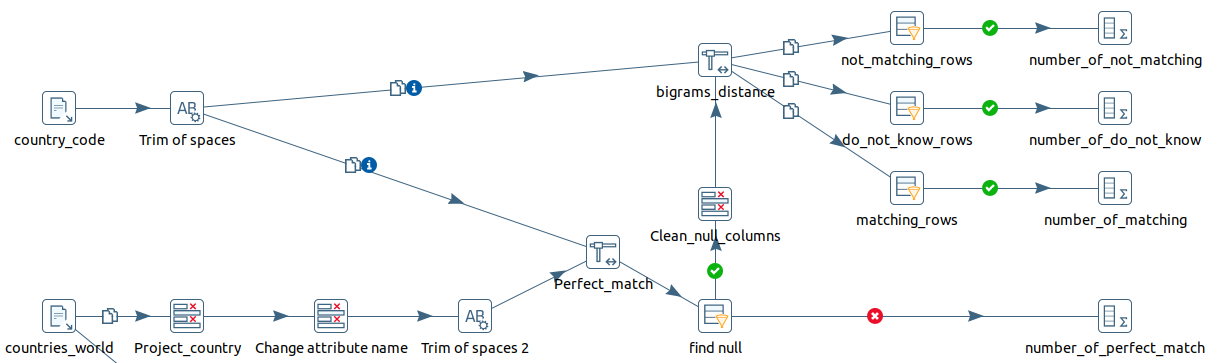
\includegraphics[width=0.7\linewidth]{images/DQ_countrycodeaccuracy}
	\caption{Pipeline per il conteggio delle tuple con codice di Country non valido.}
	\label{fig:dqcountrycodeaccuracy}
\end{figure}

\subsection{Completezza del dataset delle nazioni}
\label{subsec:compl_country}
La completezza analizzata è la completezza per attributo, in particolare abbiamo utilizzato la definizione “standard”, ovvero:\\“il numero di valori  \texttt{null} che compaiono nella colonna di un attributo.”.\\
Stando alla definizione, non abbiamo ricercato possibili valori non \texttt{null} ma i quali non possegono valori semantici corretti rispetto all'attributo.
Questa casistica è stata analizzata e studiata per la parte di integrazione dei dati, ma non per la parte di completezza, poiché ci siamo limitati alla definizione di completezza. 
In Tabella \ref{tab:compl_country} sono presenti il numero, e relativa percentuale, dei valori \texttt{null} per ogni colonna, infine, si è contato anche il numero complessivo di valori nulli e la loro percentuale rispetto al totale.
Dalle misure effettuate, realizzate grazie alla pipeline mostratta in Figura \ref{fig:dqcompletezzacountry}, possiamo dire che il dataset è praticamente completo, soprattutto riguardo al GDP che è un attributo che verrà utilizzato per la parte di apprendimento automatico.
\begin{table}
	\caption{Tabella riassuntiva contenente numero e percentuale (si ricorda che si hanno 227 nazioni) dei valori a \texttt{null} presenti nel dataset per ogni attributo. Infine, si fornisce un'ultima riga contenente il numero totale di \texttt{null} e la percentuale rispetto alla somma dei campi del dataset.}
	
	\label{tab:compl_country}
	
	\centering
	\begin{tabular}{|c|c|c|}
		\hline
		\textbf{Attributo}  & \textbf{Numero} & \textbf{Percentuale (\%)} \\ 
		\hline  
		\rule{0pt}{13pt}Country & 0 & 0 \\ 
		\hline  
		\rule{0pt}{13pt}Region & 0  & 0 \\ 
		\hline  
		\rule{0pt}{13pt}Population & 0 & 0 \\ 
		\hline  
		\rule{0pt}{13pt}Area & 0 & 0 \\ 
		\hline
		\rule{0pt}{13pt}Pop. Density & 0 & 0 \\
		\hline
		\rule{0pt}{13pt}Coastline & 0 & 0 \\
		\hline
		\rule{0pt}{13pt}Net migration & 3 & 1 \\
		\hline
		\rule{0pt}{13pt}Infant mortality & 3 & 1 \\
		\hline
		\rule{0pt}{13pt}GDP & 1 & 0.4 \\
		\hline
		\rule{0pt}{13pt}Literacy & 18 & 8 \\
		\hline
		\rule{0pt}{13pt}Phones & 4 & 2 \\
		\hline
		\rule{0pt}{13pt}Arable & 2 & 1 \\
		\hline
		\rule{0pt}{13pt}Crops & 2 & 1 \\
		\hline
		\rule{0pt}{13pt}Other & 2 & 1 \\
		\hline
		\rule{0pt}{13pt}Climate & 22 & 10 \\
		\hline
		\rule{0pt}{13pt}Birthrate & 3 & 1 \\
		\hline
		\rule{0pt}{13pt}Deathrate & 4 & 2 \\
		\hline
		\rule{0pt}{13pt}Agriculture & 15 & 7 \\
		\hline
		\rule{0pt}{13pt}Industry & 16 & 7 \\
		\hline
		\rule{0pt}{13pt}Service & 15 & 7 \\
		\hline   
		\rule{0pt}{13pt}\textbf{Totale} & \textbf{110} & \textbf{2.4} \\
		\hline
	\end{tabular}
\end{table}

\begin{figure}
	\centering
	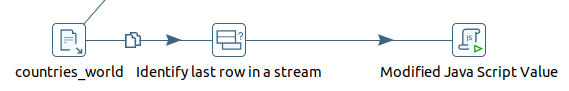
\includegraphics[width=0.7\linewidth]{images/DQ_completezzacountry}
	\caption{Pipeline che utilizza uno script Javascript (cfr. Appendice A) per verificare la completezza del campo Country.}
	\label{fig:dqcompletezzacountry}
\end{figure}


\subsection{Accuratezza sintattica del codice delle nazioni del dataset Kickstarter}
Per quanto concerne l'accuratezza sintattica delle nazioni nel dataset dei kickstarter (le quali sono rappresentate dal codice a due cifre), prima di verificarne l'accuratezza sintattica,in un modo analogo a come fatto per il dataset precedente, abbiamo valutato quanti valori univoci dell'attributo comparissero e quanti di questi avessero un match esatto con un codice del dizionario, i risultati sono riportati in Tabella \ref{tab:unique_code_country}.
Analizzando i numeri appena riportati in tabella, è stato necessario capire perché comparisse un così alto numero di valori univoci che non riportavano match: andando a valutare la lista dei valori univoci assunti da quell'attributo, abbiamo notato che tutti i non match sono stati causati dall'assunzione di un valore sintatticamente sbagliato da parte dell'attributo (\textit{i.e.}, numeri o stringhe più lunghe di due caratteri); al contempo non vi erano codici di due cifre che non presentavano un match con il dizionario di riferimento.

\begin{table}
	\caption{Nella prima riga è presente il numero di codici univoci che hanno un match esatto con un codice a due cifre del dizionario di riferimento, nella seconda riga, invece, i codici che non presentano un match esatto.}
	
	\label{tab:unique_code_country}
	
	\centering
	\begin{tabular}{c|c}
		Match & 21\\ 
		Non match & 141 \\
	\end{tabular}
\end{table} 

In seguito, abbiamo misurato l'accuratezza sintattica dei codici sfruttando il dizionario utilizzato nella fase precedente: dato che i codici sono composti da due sole cifre, abbiamo deciso di utilizzare la distanza di edit e di cercare solo i match perfetti, il numero di tuple con un codice di nazione sintatticamente valido e quelle con un codice non valido (cioè che non compariva nel dizionario) sono state riportate in Tabella \ref{tab:code_country_compl}.
A fronte di quello riportato in tabella e tenendo presente la distribuzione dei valori univoci tra match e non match, siamo giunti alla conclusione che nonostante i non match abbiano un numero di valori univoci estremamente maggiore, l'accuratezza sintattica rimane elevata perché quei valori compaiono poche volte all'interno del dataset e sono causati, probabilmente, dalla mancanza di informazioni su questo attributo o da un problema proveniente da di chi ha generato il dataset. 
Di conseguenza, facendo riferimento alla Tabella \ref{tab:code_country_compl} possiamo affermare che il dataset è accurato sintatticamente e che queste poche tuple scorrette verranno eliminate durante il processo di data integration, non consideriamo l'ipotesi di sistemarle poiché risulterebbe molto costoso come processo ed il dataset rimane comunque più che sufficiente per la parte di apprendimento automatico.\\
L'intera pipeline è mostrata in Figura \ref{fig:dqaccuratezzacodicenazioni}.

\begin{table}
	\caption{Nella prima riga è presente il numero e la relativa percentuale di tuple (ricordando che in totale si hanno 323750 tuple) che hanno un match con un codice a due cifre del dizionario di riferimento, nella seconda riga, invece, le tuple che non hanno un match.}
	
	\label{tab:code_country_compl}
	
	\centering
	\begin{tabular}{c|cc}
		Match & 319328 & 98.6 \% \\ 
		Non match & 4422 & 1.4 \% \\
	\end{tabular}
\end{table} 

\begin{figure}
	\centering
	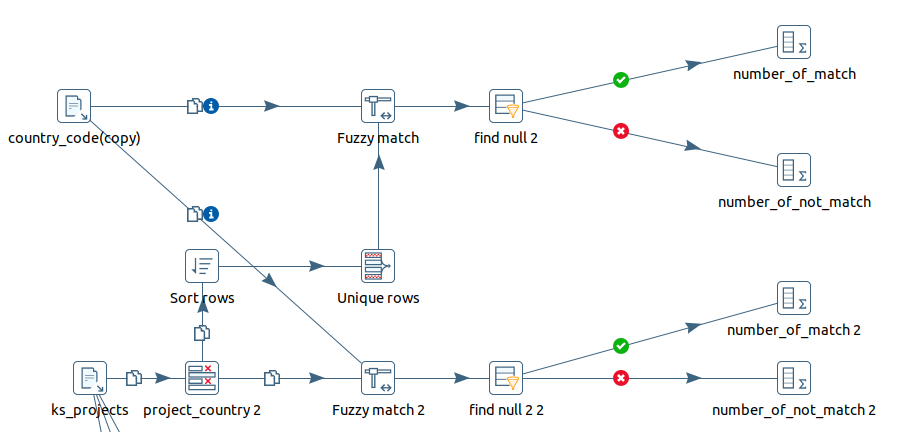
\includegraphics[width=0.7\linewidth]{images/DQ_accuratezzacodicenazioni}
	\caption{Pipeline che realizza la misura di accuratezza sintattica per l'attributo Country del dataset dei Kickstarter.}
	\label{fig:dqaccuratezzacodicenazioni}
\end{figure}


\subsection{Accuratezza sintattica attributo State}
Poiché l'attributo State sarà l'attributo soggetto alla predizione dei modelli di apprendimento automatico che verranno sviluppati, è stato necessario, quindi, analizzare la sua accuratezza sintattica.
Gli unici valori validi sintatticamente sono: successful, failed, canceled, live e suspended; dato che i valori sono di un numero ridotto, le tuple con un valore non valido sono state filtrate mediante l'utilizzo di una \textit{query}, senza applicare, quindi, delle misure di distanza con il dizionario. 
Tale operazione è stata possibile grazie ad uno studio preliminare dei valori univoci assunti da tale attributo, i cui risultati sono riportati in Tabella \ref{tab:unique_state}.
Dei 405 valori non validi, 404 sono numeri o date e l'ultimo è la stringa “undefined”, che agli scopi della nostra analisi è considerata scorretta, perché non utile, anzi fuorviante, per il processo di apprendimento automatico. 
\begin{table}
	\caption{Tabella che rappresenta il numero di valori univoci sintatticamente validi e sintatticamente non validi presenti nel dataset.}
	
	\label{tab:unique_state}
	
	\centering
	\begin{tabular}{c|c}
		Validi & 5\\ 
		Non validi & 405 \\
	\end{tabular}
\end{table} 
Il numero di tuple con un attributo state valido, e la relativa percentuale, sono riportate in Tabella \ref{tab:acc_state}.
Anche in questo caso, possiamo considerare il dataset accurato perché la percentuale di tuple con un valore valido è estremamente alto e l'eliminazione delle tuple con un campo non valido, quindi su cui non è possibile fare predizione, rimane irrilevante per il processo di estrazione di \textit{features} e apprendimento automatico.
Si faccia riferimento alla Figura \ref{fig:dqstateaccuracy}, per com'è stata definita la pipeline.
\begin{table}
	\caption{Nella prima riga è presente il numero e la relativa percentuale di tuple (ricordando che in totale si hanno 323750 tuple) che hanno un attributo State valido (ovvero uguale a: successful, failed, canceled, live e suspended), nella seconda le tuple con un valore non valido.}
	
	\label{tab:acc_state}
	
	\centering
	\begin{tabular}{c|cc}
		Validi & 319563 & 98.7 \% \\ 
		Non validi & 4187 & 1.3 \% \\
	\end{tabular}
\end{table} 

\begin{figure}[h!]
	\centering
	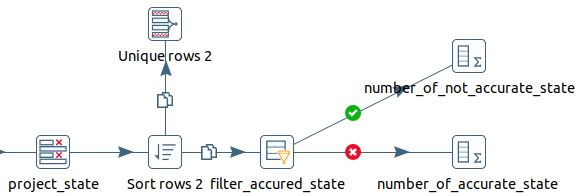
\includegraphics[width=0.7\linewidth]{images/DQ_stateaccuracy}
	\caption{Pipeline che verifica tutti i possibili valori dell'attributo State. Gli unici valori plausibili e accettati sono: successful, failed, canceled, live e suspended.}
	\label{fig:dqstateaccuracy}
\end{figure}
\newpage
\subsection{Consistenza attributo State}
Il valore dell'attributo State di una tupla deve essere successful se e solo se la differenza tra l'ammontare di soldi \textit{pledgiati} ed il goal è maggiore o uguale a zero.
Partendo da questo vincolo, abbiamo misurato il numero di tuple aventi una differenza positiva ed il cui stato non è successful; inoltre, abbiamo misurato anche il caso la cui differenza è negativa ed il cui stato è successful.
Infine, abbiamo calcolato anche i dati complementari ai primi due, ovvero quando la differenza è positiva e lo stato è successful e quando è negativa e lo stato non è successful.
Si sottolinea, che i dati riportati nella Tabella \ref{tab:cons_state} sono stati misurati sulla porzione di dataset avente dei valori numerici per i campi Pledged e Goal ed un valore di stato pari a successful, canceled e failed, perché le tuple con altri valori non verranno utilizzate per il processo di apprendimento automatico; queste azioni preliminari di filtraggio hanno in totale rimosso 10367 tuple, ovvero il 3 \% del dataset di partenza. 
Sia i risultati delle azioni di filtraggio, sia le misure riportate in Tabella \ref{tab:cons_state} evidenziano ancora una volta che il dataset è buono ed è complessivamente consistente rispetto all'attributo soggetto alla predizione.
Si faccia riferimento alla Figura \ref{fig:dqstateaconsistency} per la relativa pipeline.
\begin{table}
	\caption{Tabella riassuntiva della consistenza dell'attributo State, basandosi sulla differenza tra soldi \textit{pledgiati} ed il goal. Se tale differenza è maggiore o uguale a zero, l'attributo State deve essere successful; al contrario se la differenza è minore o uguale a zero, il valore non deve essere successful.}
	
	\label{tab:cons_state}
	
	\centering
	\begin{tabular}{c|cc}
		& $n^{\circ}$ successful & $n^{\circ}$ non successful \\
		\hline
		\rule{0pt}{13pt}Differenza $\geq 0$  & 112960 & 519 \\ 
		\rule{0pt}{13pt}Differenza $< 0$& 5 & 199899 \\
	\end{tabular}
\end{table} 
\begin{figure}[h!]
	\centering
	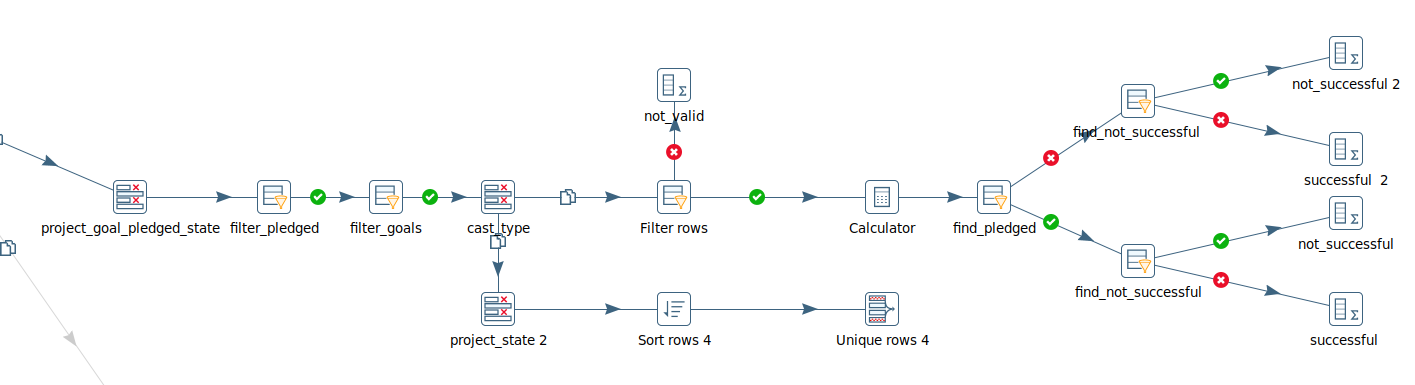
\includegraphics[width=0.7\linewidth]{images/DQ_stateaconsistency}
	\caption{Pipeline per il conteggio delle tuple il cui valore dell'attributo State non è consistente con il totale del denaro raccolto.}
	\label{fig:dqstateaconsistency}
\end{figure}

\newpage
\subsection{Consistenza attributo Backers}
\label{subsec:cons_backers}
Il vincolo di consistenza sull'attributo Backers è che il loro valore deve essere maggiore di zero se e solo il valore dell'attributo Pledged è maggiore di zero.
Per verificare ciò, sono state prima rimosse tutte le tuple aventi un valore di Backers sintatticamente non valido (\textit{i.e.}, numero negativo o una stringa) e successivamente verificato il vincolo sopra citato.
I risultati di tale metrica sono riportati in Tabella \ref{tab:con_backers}, si fa presente che 624 tuple delle 3703 non valide sono le tuple aventi un valore dell'attributo sintatticamente non valido.
Anche in questo secondo caso si può considerare il dataset consistente ed accurato rispetto all'attributo Backers.
La pipeline è rappresentata in Figura \ref{fig:dqbackersconsistency}.

\begin{table}
	\caption{Nella prima riga è presente il numero e la relativa percentuale di tuple (ricordando che in totale si hanno 323750 tuple) che hanno un attributo Backers che soddisfa il vincolo di integrità, nella seconda il numero di tuple che non lo soddisfano.}
	
	\label{tab:con_backers}
	
	\centering
	\begin{tabular}{c|cc}
		Validi & 320047 & 98.9 \% \\ 
		Non validi & 3703 & 1.1 \% \\
	\end{tabular}
\end{table} 

\begin{figure}[h!]
	\centering
	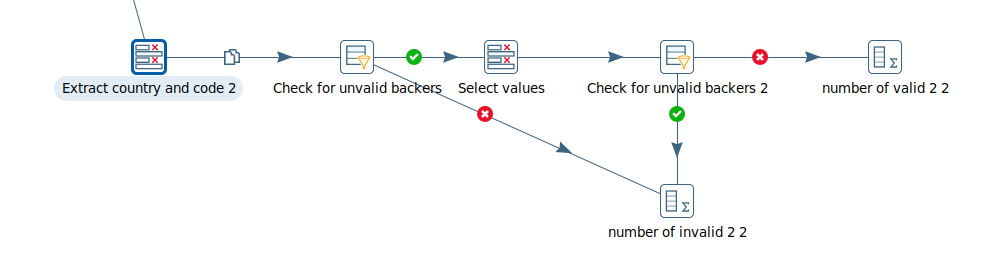
\includegraphics[width=0.7\linewidth]{images/DQ_backersconsistency}
	\caption{Pipeline per il conteggio delle tuple il cui valore dell'attributo Backers assume un valore negativo oppure non è consistente con il totale del denaro raccolto.}
	\label{fig:dqbackersconsistency}
\end{figure}

\subsection{Completezza del dataset Kickstarter}
Come già detto in precedenza (Sotto sezione \ref{subsec:compl_country}), per completezza intendiamo: “il numero di valori  \texttt{null} che compaiono nella colonna di un attributo.”.
Di conseguenza anche in questo caso andiamo a valutare solo i valori \texttt{null} e non tutti quei valori, anche se presenti come già mostrato precedentemente, sintatticamente scorretti.
In Tabella \ref{tab:compl_ks} sono presenti il numero e la relativa percentuale di valori \texttt{null} per ogni colonna, infine si è contato anche il numero complessivo di valori nulli e la loro percentuale rispetto al totale.
Dalle misure effettuate, possiamo dire che il dataset è praticamente completo, inoltre il dato che manca spesso è l'ammontare in dollare dei soldi donati, il quale non è un attributo utilizzato per il processo di apprendimento automatico.
La pipeline è analoga a quella utilizzata nella Sotto sezione \ref{subsec:compl_country}, come mostrato in Figura \ref{fig:dqcompletezza}.
\begin{table}
	\caption{Tabella riassuntiva contenente numero e percentuale dei valori \texttt{null} presenti nel dataset per ogni attributo. Infine, si fornisce un'ultima riga contenente il numero totale di \texttt{null} e la percentuale rispetto ad ogni campo del dataset.}
	
	\label{tab:compl_ks}
	
	\centering
	\begin{tabular}{|c|c|c|}
		\hline
		\textbf{Attributo}  & \textbf{Numero} & \textbf{Percentuale (\%)} \\ 
		\hline  
		\rule{0pt}{13pt}ID & 0 & 0 \\ 
		\hline  
		\rule{0pt}{13pt}Name & 0  & 0 \\ 
		\hline  
		\rule{0pt}{13pt}Category & 5 & {\raise.17ex\hbox{$\scriptstyle\sim$}}0 \\ 
		\hline  
		\rule{0pt}{13pt}Main category & 0 & 0 \\ 
		\hline
		\rule{0pt}{13pt}Currency & 0 & 0 \\
		\hline
		\rule{0pt}{13pt}Deadline & 0 & 0 \\
		\hline
		\rule{0pt}{13pt}Goal & 0 & 0 \\
		\hline
		\rule{0pt}{13pt}Launched & 0 & 0 \\
		\hline
		\rule{0pt}{13pt}Pledged & 0 & 0 \\
		\hline
		\rule{0pt}{13pt}State & 0 & 0 \\
		\hline
		\rule{0pt}{13pt}Backers & 0 & 0\\
		\hline
		\rule{0pt}{13pt}Country & 0 & 0 \\
		\hline
		\rule{0pt}{13pt}Usd pledged & 3790 & 1.1 \\
		\hline
		\rule{0pt}{13pt}\textbf{Totale} & \textbf{3795} & \textbf{0.09} \\
		\hline
	\end{tabular}
\end{table}

La profilazione dei dati eseguita in precedenza ha mostrato possibili casi di valori sintatticamente corretti ma semanticamente errati; in particolare, un piccolo sottoinsieme di tuple (circa 500) ha mostrato valori privi di senso in diversi campi. Questo sottoinsieme di tuple è stato rimosso dalle operazioni di trasformazione eseguite successivamente, ed è quindi stato deciso di non includere il conteggio di queste tuple nell'analisi della completezza

\begin{figure}
	\centering
	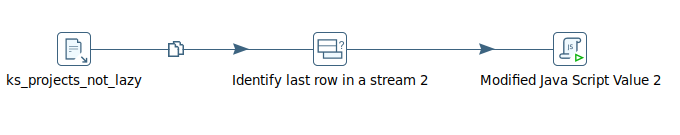
\includegraphics[width=0.7\linewidth]{images/DQ_completezza}
	\caption{Pipeline che utilizza uno script Javascript custom (cfr. Appendice A) che itera sui campi del dataset e conta il numero di tuple con valore dell'attributo nullo.}
	\label{fig:dqcompletezza}
\end{figure}

\subsection{Accessibilità dei dataset}
Tutti i dataset analizzati mostrano un ottimo livello di accessibilità da parte dell'utente, con nomi degli attributi autoesplicativi e facile reperibilità dei dati di interesse. 
Le uniche note negative di quanto appena detto sono i valori dell'attributo \textit{Climate}, poiché sono dei numeri la cui semantica non è stata specificata, inoltre l'attributo \textit{Coastline}, seppur intuitivo, non è chiaro come sia stato calcolato, si è supposto essere il rapporto tra area costiera e non costiera, ma non si ha la certezza; potrebbe sorgere anche la domanda di come sia definita formalmente l'area costiera.
Dato che nel complesso la leggibilità risulta alta ed i problemi di accessibilità riguardano prettamente la semantica del dato e non nel nome dell'attributo, non si è resa necessaria la creazione di viste sugli schemi locali dei dataset, mantenendo inalterata la struttura di questi ultimi.

\subsection{Porprietà temporali}
\label{subsec:temporali}
Il dataset \textit{ks-projects-201612.csv} contiene tutti i progetti registrati sulla piattaforma Kickstarter fino alla fine del 2016. Il dataset \textit{countries of the world.csv} contiene invece statistiche sugli stati che si riferiscono all'anno 2017. Ne consegue che i dati non siano perfettamente coerenti dal punto di vista temporale, ma abbiamo reputato questo sfasamento marginale, considerata l'assenza di modifiche radicali degli indici statistici inerenti alle nazioni presi in considerazioni in anni consecutivi.
Inoltre, per quanto concerne il valore di aggiornamento dei dati, i dataset utilizzati non soddisfano pienamente tale misura, in quanto ci si aspetterebbe di disporre dei dati relativi all'anno 2018.

\newpage
\section{Processo di integrazione dei dati}
Al fine di produrre un dataset integrato per il processo di Machine Learning, si è reso necessario unire i tre dataset scelti in un unico schema integrato. Prima di fare ciò, sfruttando le considerazioni fatte nella parte di analisi di qualità dei dati, sono state eseguite una serie di operazioni di pulizia e raffinamento dei dati.\\

\begin{figure}
	\hspace*{-1cm}%
	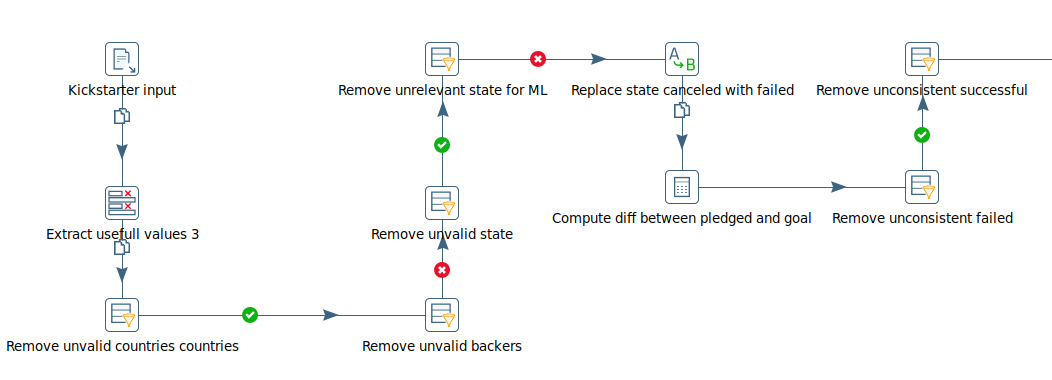
\includegraphics[width=\dimexpr\textwidth+2cm\relax]{images/transformation_kick}%
	\hspace*{-1cm}%
	\caption{Pipeline di trasformazione per il dataset contenente i dati dei progetti Kickstarter.}
	\label{fig:transformationkick}
\end{figure}

\subsection{Dataset Kickstarter}
Inizialmente sono stati eliminati tutti quegli attributi che non avevano alcuna informazione rilevante ai fini del training del modello di Machine Learning (Data di creazione e di terminazione, nome, moneta utilizzata \dots).\\
In seguito, sono stati rimossi tutti quei record il cui campo relativo alla nazione di origine violasse la rappresentazione standard, ovvero due lettere dell'alfabeto maiuscole. Ciò si è reso necessario in quanto l'analisi della accuratezza sintattica sul campo aveva mostrato una serie di valori privi di significato, evidenzando anche il fatto che tutti i codici sintatticamente validi avessero un corrispettivo nel dataset utilizzato come dizionario.\\
Sono stati poi rimossi una serie di record che creavano problemi di consistenza per quanto riguarda il campo dei sostenitori e del totale raccolto. Le analisi condotte in precedenza avevano, infatti, rilevato che alcuni record avevano un numero di sostenitori negativo, oppure un numero di sostenitori pari a zero, ma il campo che rappresenta l'ammontare del denaro raccolto non era zero anch'esso.\\
È stata poi condotta un'operazione di raffinazione sul campo State del dataset, che rappresenta lo stato in cui il progetto si trova. Dopo aver rimosso tutti i valori sintatticamente privi di senso, abbiamo deciso di rimuovere tutti i record il cui stato fosse live, ovvero ancora in corso, oppure suspended, ovvero bloccati dalla piattaforma Kickstarter per violazioni dei termini contrattuali. Questa decisione è stata presa in quanto questo tipo di record potrebbe influenzare negativamente le performance del modello di Machine Learning, fornendo tuple con uno stato non ben determinato.
È stato, poi, deciso di unificare i valori failed e canceled (ovvero le campagne cancellate dal creatore) dell'attributo State, rendendo tale attributo pari a failed per tutte le tuple aventi lo stato pari a canceled.\\
Infine, sono stati rimossi tutti i record che mostravano inconsistenza tra lo stato del progetto e la differenza tra denaro richiesto e denaro raccolto. È infatti mandatorio che se è stato raccolto più denaro di quanto richiesto, il progetto risulti completato, mentre se non sono stati raccolti fondi insufficienti, il progetto risulti fallito.\\
L'intera pipeline di trasformazione è riportata in Figura \ref{fig:transformationkick}.


\subsection{Countries}
Siccome il dataset contenente i dettagli sui progetti Kickstarter sfrutta il codice di 2 lettere per rappresentare la nazione di origine del progetto, mentre il dataset con le informazioni circa il livello di sviluppo dei vari Paesi sfrutta il nome completo, è stato necessario individuare un terzo dataset da utilizzare come una tabella di join, in modo da associare ogni nome per esteso con il relativo codice di due lettere.\\
Il dataset individuato per questo scopo si è però rivelato utilizzare una differente sintassi per rappresentare il nome per esteso di alcuni Paesi. Per questo motivo, sono state applicate delle tecniche di \textit{record linkage} per individuare i record corrispondenti ed uniformare la sintassi di questi. Per fare ciò, sono stati utilizzati i dati prodotti dal processo di analisi di qualità dei dati (trattato nella prima parte di questo documento).\\
In particolare, sono stati ignorati i record di perfect match prodotti dalla distanza di edit con soglia zero, mentre sono stati confrontati caso per caso i risultati prodotti dall'analisi tramite Bigram. Ponendo la soglia di match a 0.7 e la soglia di non match a 0.5, la soluzione proposta ha prodotto performance ottime, individuando correttamente tutti i match (20/20), e buona parte dei non match(7/11). La presenza di casi limite, quali rappresentazioni radicalmente diverse di un medesimo record, ha reso necessario la supervisione manuale di questi record, permessa dal fatto che nel complessivo i record analizzati con le Bigram erano pochi e facilmente confrontabili. La pipeline per l'esecuzione del \textit{record linkage} è riportata in Figura \ref{fig:recordlinkage}.\\

\begin{figure}
	\centering
	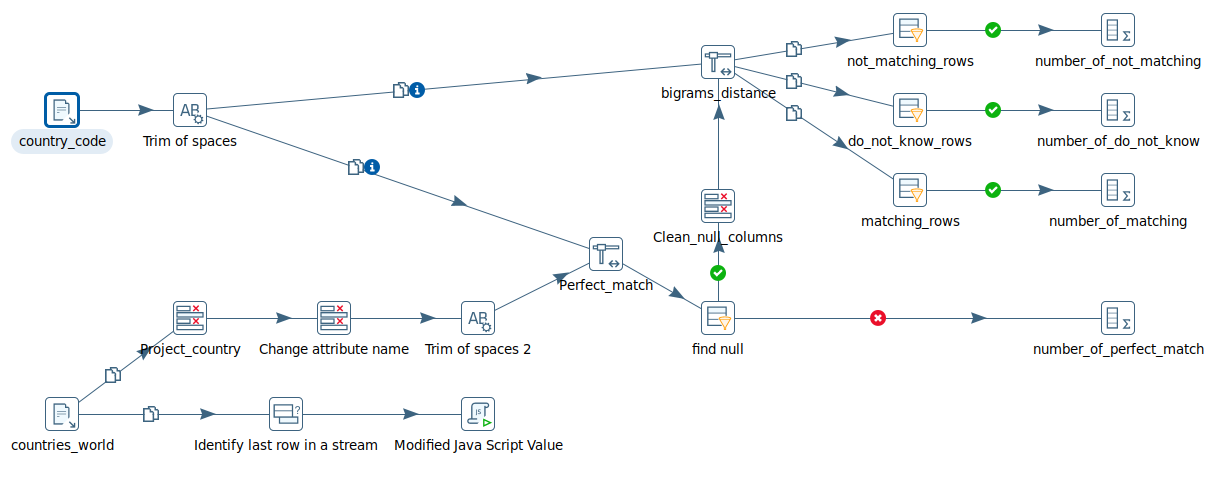
\includegraphics[width=0.7\linewidth]{images/RecordLinkage}
	\caption{Pipeline eseguita per realizzare le operazioni di \textit{record linkage}.}
	\label{fig:recordlinkage}
\end{figure}

\newpage
\section{Produzione dataset integrato}
A seguito del processo di raffinamento e integrazione dei dataset esposto in precedenza, i tre dataset sono stati uniti in un'unica tabella tramite delle operazioni di \textit{merge join}, per motivi di efficienza.\\
A seguito della fusione, sono stati prodotti due nuovi dataset (come mostrato in Figura \ref{fig:transformationcomplete}), uno contenente tutti gli attributi risultanti dalle operazioni precedenti, mentre l'altro epurato da tutti gli attributi privi di valore ai fini dell'addestramento del modello di Machine Learning. Si sottolinea che anche il primo dataset è figlio di operazioni di pulizia di attributi, quindi non contiene tutti gli attributi dei due dataset iniziali; a questo punto, la creazione di un dataset del tipo di quello appena descritto risulta triviale da effettuare.

\begin{figure}[p!]
	\centering
	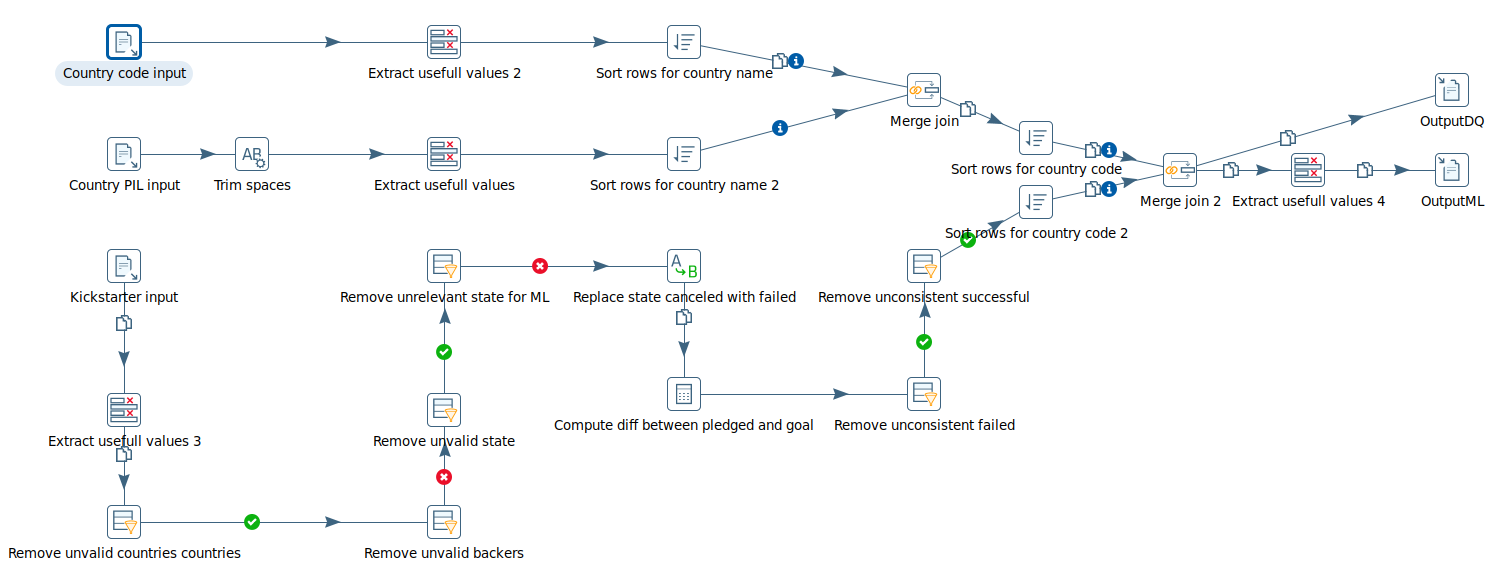
\includegraphics[angle=90,origin=c,height=1.1\linewidth]{images/transformation_complete}
	\caption{Pipeline di trasformazione per il dataset contenente i dati dei progetti Kickstarter.}
	\label{fig:transformationcomplete}
\end{figure}

\newpage
\section{Analisi di qualità dei dataset (post-integrazione)}
Al fine di valutare la qualità del lavoro svolto nella fase di integrazione del dataset, le misure di qualità precedentemente stabilite sono state applicate al dataset integrato. In questa sezione verranno riportati i risultati ottenuti e le relative considerazioni.

\subsection{Accuratezza sintattica attributo Country}
Per la misura dell'accuratezza sintattica è stata utilizzata la pipeline mostrata in Figura \ref{fig:dqtcountries}, che individua le tuple il cui valore dell'attributo Country risulta sintatticamente insensato e conta i possibili valori che questo campo assume.\\
L'attributo presenta 21 possibili valori, tutti formati da una coppia di 2 lettere maiuscole dell'alfabeto. Non sono presenti tuple con valore dell'attributo che violino questo vincolo sintattico.

\begin{figure}[h!]
	\centering
	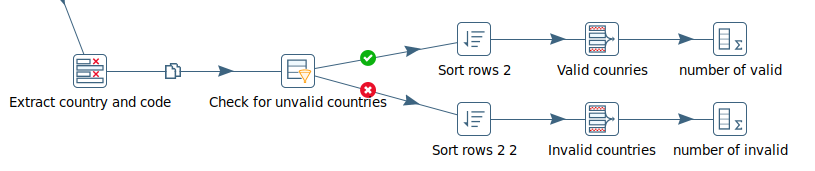
\includegraphics[width=1\linewidth]{images/DQT_countries}
	\caption{Pipeline per la verifica della accuratezza sintattica dell'attributo Country.}
	\label{fig:dqtcountries}
\end{figure}


\subsection{Accuratezza sintattica attributo State}
L'attributo State risulta assumere due possibili valori: successful e failed. Le trasformazioni applicate producono quindi una riduzione dei possibili valori da 410 a 2 possibili valori.

\subsection{Consistenza attributo State}
Per l'attributo in esame, non sono presenti tuple inconsistenti, ove il totale raccolto non sia consistente con lo stato del progetto. La pipeline in Figura \ref{fig:dqtstate} mostra la ricerca dei possibili valori del campo State ed il conteggio di eventuali tuple con valore dell'attributo state non consistenti con il totale raccolto.

\begin{figure}[h!]
	\centering
	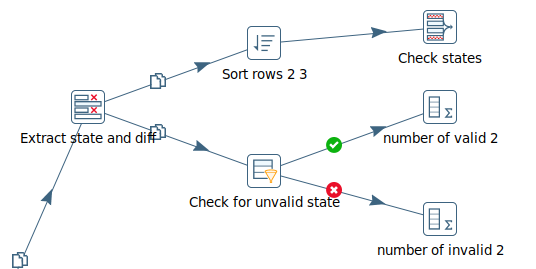
\includegraphics[width=0.6\linewidth]{images/DQT_state}
	\caption{Pipeline per la verifica della consistenza e della accuratezza sintattica dell'attributo State}
	\label{fig:dqtstate}
\end{figure}

\subsection{Consistenza attributo Backers}
Per il campo Backers, è stata realizzata una pipeline (mostrata in Figura \ref{fig:dqtbackers}) con l'intento di individuare eventiali tuple che violassero i vincoli di consistenza. La verifica si è concentrata sul valore del campo Backers in relazione con il totale del denaro riscosso, basandosi sul vincolo definito nella Sotto sezione \ref{subsec:cons_backers}.\\
L'esecuzione della pipeline non ha portato alla rilevazione di tuple che violassero i vincoli imposti.

\begin{figure}[h!]
	\centering
	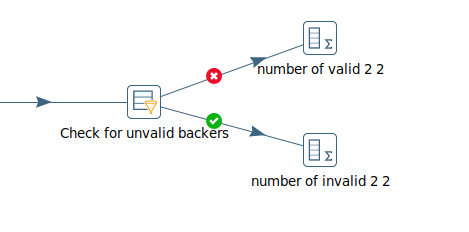
\includegraphics[width=0.7\linewidth]{images/DQT_backers}
	\caption{Pipeline per la verifica della consistenza dell'attributo backers}
	\label{fig:dqtbackers}
\end{figure}

\subsection{Completezza del dataset}
Ai fini di valutare la completezza del dataset prodotto, è stato eseguito nuovamente lo script riportato in Appendice A, che ricerca e conta i campi nulli presenti del dataset. L'esecuzione di questo processo conferma l'assenza di campi nulli nel dataset prodotto.

\subsection{Accessibilità del dataset}
Al fine di garantire un'accessibilità ottimale al dataset sfruttato per eseguire il training dei modelli di Machine Learning, sono stati selezionati nomi significativi ed autoesplicativi per gli attributi presenti nel dataset integrato.

\subsection{Porprietà temporali}
Le considerazioni relative alle proprietà temporali rimangono analoghe a quelle effettuate prima delle operazioni di integrazione dei dati.

\subsection{Altre misure di qualità}
Al fine di verificare l'efficacia dell'operazione di \textit{record linkage} e \textit{data fusion} (eseguite “a mano”) compiute sul campo Country del dataset \textit{countries of the world}, sono state nuovamente misurate le distanze con il campo Country name del dataset \textit{country\_code}. Questa misura, eseguita mediante la pipeline riportata in Figura \ref{fig:qdtrecordlinkage}, mostra come il numero dei match esatti sia aumentato a seguito delle modifche apportate al dataset \textit{countries of the world}. Allo stesso modo, sfruttando la distanza con le Bigram, all'interno degli insiemi di incertezza e di non match, sono rimaste solo le coppie che effettivamente non dovevano essere \textit{linkate}, mentre quelle rilevate come match nella prima analisi sono state tutte portate ad essere match esatti.\\
In Tabella \ref{tab:recap} si mostrano il numero di tuple che non soddisfano i vincoli di consistenza o di accuratezza sintattica prima e dopo le trasformazioni applicate; si riportano le metriche di qualità relative al dataset contenente le informazioni dei Kickstarter.
\begin{figure}[h!]
	\centering
	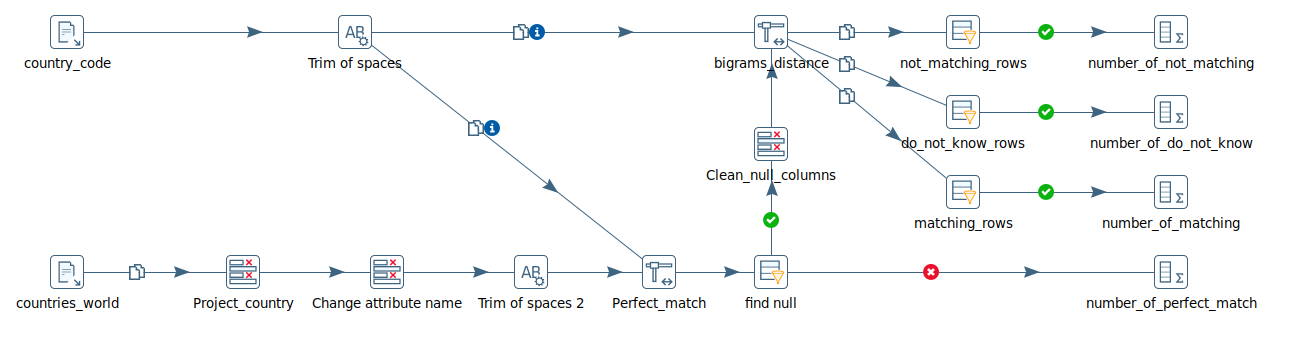
\includegraphics[width=1\linewidth]{images/QDT_recordlinkage}
	\caption{Pipeline utilizzata per la verifica del processo di \textit{record linkage} effettuata}
	\label{fig:qdtrecordlinkage}
\end{figure}
	\begin{table}
		\caption{Tabella riassuntiva che mostra il numero di tuple che non soddisfano i vincoli di consistenza o di accuratezza sintattica prima e dopo le trasformazioni applicate. Si noti che della ocmpletezza si riporta il numero totale di valori di attributi che assumono il valore \texttt{null}.}
	
		\label{tab:recap}
	
		\centering
	\begin{tabular}{|c|c|c|}
		\hline 
		\textbf{Misura} & \textbf{Pre-trasformazione} & \textbf{Post-trasformazione} \\ 
		\hline 
		Accuratezza sintattica Country & 141 & 0 \\ 
		\hline
		Accuratezza sintattica State & 404 & 0 \\ 
		\hline 	
		Consistenza State & 524 & 0 \\ 
		\hline 
		Consistenza Backers & 3703 & 0 \\ 
		\hline 
		Completezza dataset & 3795 & 0 \\ 
		\hline 
	\end{tabular} 
\end{table}
\newpage
\section{Analisi descrittiva dei dati integrati}
Le analisi descrittive che si sono ritenute importanti per il dataset integrato, il quale è stato ripulito da un insieme di campi non utili per il processo di Machine Learning, sono di seguito riportate.
In particolare:
\begin{itemize}
	\item in Tabella \ref{tab:prj_country} riportiamo il numero di campagne per ogni nazione e la loro distribuzione;
	\item in Tabella \ref{tab:prj_succ_nosucc} riportiamo il numero di campagne che hanno avuto successo e che non lo hanno avuto per ogni nazione;
	\item in Tabella \ref{tab:succ_mean_sd} riportiamo la media, e deviazione standard, del goal e dell'ammontare \textit{pledgiato} delle campagne che hanno avuto successo, per ogni percentuale (che compare nel dataset) di diffusione del settore terziario nella nazione; 
	\item in Tabella \ref{tab:fail_mean_sd} riportiamo la media, e deviazione standard, del goal e l'ammontare pledgiato delle campagne fallite, per ogni percentuale (che compare nel dataset) di diffusione del settore terziario nella nazione.
\end{itemize} 

\begin{table}
	\caption{Tabella contenente per ogni nazione il numero di campagne avviate e la relativa percentuale, i dati sono stati calcolati sul dataset integrato. Si noti che le percentuali sono state arrotondate.}
	
	\label{tab:prj_country}
	
	\centering
	\begin{tabular}{|c|c|c|}
		\hline
		\textbf{Nazione} & \textbf{$\mathbf{n^{\circ}}$ campagne} & \textbf{Percentuale}\\
		\hline
		Australia & 6020 & 1.9 \\
		\hline
		Austria & 345 & 0.1 \\
		\hline
		Belgium & 379 & 0.1\\
		\hline
		Canada & 11628 & 3.7\\
		\hline
		Denmark & 783 & 0.2\\
		\hline
		France & 1792 & 0.5\\
		\hline
		Germany & 2530 & 0.8\\
		\hline
		Hong Kong & 61 & {\raise.17ex\hbox{$\scriptstyle\sim$}}0\\
		\hline
		Ireland & 549 & 0.1\\
		\hline
		Italy & 1622 & 0.5\\
		\hline
		Luxembourg & 35 & {\raise.17ex\hbox{$\scriptstyle\sim$}}0\\
		\hline
		Mexico & 16 & {\raise.17ex\hbox{$\scriptstyle\sim$}}0\\
		\hline
		Netherlands & 2187 & 0.6\\
		\hline
		New Zealand & 1106 & 0.3\\
		\hline
		Norway & 505 & 0.1\\
		\hline
		Singapore & 78 & {\raise.17ex\hbox{$\scriptstyle\sim$}}0\\
		\hline
		Spain & 1277 & 0.4\\
		\hline
		Sweden & 1211 & 0.4\\
		\hline
		Switzerland & 433 & 0.1\\
		\hline
		United Kingdom & 26882 & 8.5\\
		\hline
		United States & 253456 & 81\\
		\hline
	\end{tabular}
\end{table}

\begin{table}
	\caption{Tabella contenente per ogni nazione il numero di campagne che hanno avuto successo e quelle fallite, i dati sono stati calcolati sul dataset integrato.}
	
	\label{tab:prj_succ_nosucc}
	
	\centering
	\begin{tabular}{|c|c|c|}
		\hline
		\textbf{Nazione} & \textbf{$\mathbf{n^{\circ}}$ successfull} & \textbf{$\mathbf{n^{\circ}}$ failed}\\ \hline
		Australia            &1450
&4570 \\ \hline
		Austria              &60
&285 \\ \hline
		Belgium              &79
&300 \\ \hline
		Canada               &3067
&8561 \\ \hline
		Denmark              &231
&552 \\ \hline
		France               &512
&1280 \\ \hline 
		Germany              &529
&2001 \\ \hline
		Hong Kong            &14
&47 \\ \hline
		Ireland              &133
&416 \\ \hline
		Italy                &232
&1390 \\ \hline
		Luxembourg           &13
&22 \\ \hline
		Mexico               &2
&14 \\ \hline
		Netherlands          &410
&1777 \\ \hline
		New Zealand          &330
&776 \\ \hline
		Norway               &108
&397 \\ \hline
		Singapore            &32
&46 \\ \hline
		Spain                &242
&1035 \\ \hline
		Sweden               &335
&876 \\ \hline
		Switzerland          &86
&347 \\ \hline
		United Kingdom       &9340
&17542 \\ \hline
		United States        &95766 &157690 \\ \hline
	\end{tabular}
\end{table}
\newpage
\begin{table}
	\caption{Tabella contenente per ogni percentuale di diffusione del settore terziario: il goal medio, e sua deviazione standard (D.S.), l'ammontare medio \textit{pledgiato}, e sua D.S., delle campagne che hanno avuto successo; si noti che l'analisi è stata effettuata sul dataset integrato.}
	
	\label{tab:succ_mean_sd}
	
	\centering
	\begin{tabular}{|c|c|c|c|c|}
		\hline
		\textbf{Nazione} & \textbf{Media Goal} & \textbf{D.S. Goal} & \textbf{Media Pledged} & \textbf{D.S. Pledged} \\ \hline
		0.5&10268&22595&14428&29469 \\ \hline
		0.6&38433&60519&81987&233728
\\ \hline
		0.7&14259&36882&32329&133966
\\ \hline
		0.8&9257&29048&20638&148090
\\ \hline
		0.9&47600&83035&106829&175487 \\ \hline
	\end{tabular}
\end{table}

\begin{table}
	\caption{Tabella contenente per ogni percentuale di diffusione del settore terziario: il goal medio, e sua deviazione standard (D.S.), l'ammontare medio \textit{pledgiato}, e sua D.S., delle campagne che hanno fallito; si noti che l'analisi è stata effettuata sul dataset integrato.}
	
	\label{tab:fail_mean_sd}
	
	\centering
	\begin{tabular}{|c|c|c|c|c|}
		\hline
		\textbf{Nazione} & \textbf{Media Goal} & \textbf{D.S. Goal} & \textbf{Media Pledged} & \textbf{D.S. Pledged} \\ \hline
		0.5&69223&512735&1097&3644 \\ \hline
		0.6&514278&5516330&3619&14537 \\ \hline
		0.7&106224&1716871&1903&13943
\\ \hline
		0.8&60798&1300938&1400&7384
\\ \hline
		0.9&238864&751142&5119&12539 \\ \hline
	\end{tabular}
\end{table}